\chapter{TESTES E AVALIAÇÃO DOS RESULTADOS}\label{CAP6}
Durante o desenvolvimento do sistema como um todo, desde a sua fase local de desenvolvimento do software até a integração com os serviços da computação em nuvem, foram feitos diversos testes para garantir que as funcionalidades básicas estipuladas no início estavam sendo atendidas. Desta forma, será abordado nesta seção como foram realizadas cada etapa dos testes, e os principais resultados obtidos.

\section{TESTE DO SOFTWARE DE LEITURA}
Depois de desenvolvido o software, foram realizados os testes de funcionalidade no ambiente de desenvolvimento (notebook) para analisar se o funcionamento estava conforme o esperado. Nesta etapa, verificou-se que algumas leituras obtidas do ELM327 estavam retornando valores que não condiziam com a realidade. Contudo, estes valores eram tratados pela biblioteca obd-java-api, disparando uma \textit{exception} da própria biblioteca referente ao valor retornado. Baseado no resultado deste teste, três hipóteses que levantadas: na primeira, possivelmente o PID referente à leitura não era suportado (ou não foi implementado) pelo veículo ou protocolo utilizado; na segunda, possivelmente por questões de segurança, o próprio sistema do veículo negou a requisição para o PID; ou ainda, poderia haver a possibilidade do dispositivo estar retornando algum dado inválido, podendo ser lixo de memória.

Depois de feita a análise do problema, foram realizados mais testes direcionados à exploração desta falha visando uma possível correção. Foi necessário também consultar a documentação do dispositivo ELM327 para entender como ele trabalhava com as solicitações. Foi descoberto que o dispositivo era capaz de retransmitir a leitura anterior, semelhante a um eco. Isso é possível pois o dispositivo contém uma pequena memória de \textit{buffer} que armazena o último comando enviado para o dispositivo. Baseando-se nestas informações coletadas, foi decidido implementar o método \textit{clearBuffer} na classe ELM327, contendo alguns comandos ‘AT’ que eram responsáveis por apagar o eco e reiniciar a comunicação, para garantir que o \textit{buffer} estivesse limpo para a nova leitura.

Após realizar a alteração proposta, foi observado que algumas das leituras que antes retornavam uma \textit{exception} estavam agora retornando valores válidos e formatados segundo a implementação da biblioteca, evidenciando que parte do problema foi solucionado. Entretanto, algumas leituras ainda continuaram a retornar as \textit{exceptions}. Baseando-se nestas observações, para as leituras que foram possíveis após a alteração mencionada, uma explicação aceitável seria a possibilidade do \textit{buffer} estar sujo. Para explicar as outras leituras que persistiram com o problema mencionado, uma das duas primeiras hipóteses poderia ser a verdadeira.

Além da questão levantada acima, observou-se também certa lentidão durante a inicialização do software e durante a realização de algumas leituras. Inicialmente foi levantado a hipótese de que a comunicação \textit{bluetooth} que estava causando a lentidão, entretanto, quando foi implementado a mesma lógica pelo console, notou-se que a execução dele foi mais rápido. Baseado neste teste, concluiu-se que a implementação contendo a interface gráfica estava deixando a execução do software mais lenta. Entretanto, apesar desta análise e conclusão, foi mantida a interface do sistema.

\section{TESTE DE INTEGRAÇÃO DO SOFTWARE COM O \textit{RASPBERRY PI}}
Depois de preparado o ambiente do \textit{Raspberry Pi}, foi executado o software no dispositivo para análise e testes. Conforme já apresentado na metodologia, foram identificadas algumas incompatibilidades, solucionadas logo na sequência. Contudo, depois das alterações, notou-se que o software foi executado mais rápido em comparação com a primeira execução no ambiente de desenvolvimento, mas ainda demorava algum tempo em alguns momentos da execução. Analisando-se o resultado dos testes, foi levantada a hipótese de a lentidão estar sendo causada pelo fato de o software estar rodando no dispositivo através da máquina virtual do Java \textit{(Java Virtual Machine – JVM)}, combinado com a renderização da interface.

A fim de tornar a execução mais rápida, foi feita uma análise técnica para estudar a viabilidade de migração do software para a linguagem \textit{Python}. Além do \textit{Raspberry} suportar scripts \textit{Python}, \citeonline{richardsonwallace} afirmam que esta linguagem tende a ser mais rápida pelo fato de ser interpretada. Durante a análise, foi encontrado uma biblioteca em \textit{Python} que trazia diversas funções que permitiam a comunicação com o ELM327, assim como a biblioteca para Java obd-java-api. Esta biblioteca para \textit{Python} foi encontrada em http://python-obd.readthedocs.io/en/latest/, junto com a documentação explicando as principais funções presentes nela. Apesar desta alternativa parecer, em primeiro momento, uma solução viável, houve alguns contratempos, que levaram a permanência do software na linguagem Java. Uma das dificuldades que tornou inviável a mudança foi o esforço demasiado grande para reestruturar todo o software na nova linguagem, considerando que todas as partes funcionais já estavam prontas em Java.

\section{TESTES DE INTEGRAÇÃO DA APLICAÇÃO COM A COMPUTAÇÃO EM NUVEM}
Após finalizada toda a parte de integração com os recursos da computação em nuvem, desde banco de dados até o \textit{web service}, foram realizados diversos testes para garantir a comunicação entre os sistemas. Nesta fase, não houve dificuldades e todo o sistema se comunicou conforme o esperado. Para garantir a comunicação do software com o banco de dados na nuvem, foi utilizada uma infraestrutura de rede móvel 4G do celular, que roteava o sinal via Wi-Fi para o \textit{Raspberry Pi}, conforme já abordado anteriormente. O teste foi realizado com o veículo em movimento, e foi notado que durante a execução, a única limitação que foi observada é que ao entrar em uma região sem cobertura 4G, o sistema não fazia upload das informações, o que resultava em perda dos dados que foram coletados. Contudo, toda informação enviada ao banco de dados era disponibilizado pelo \textit{web service} em formato de uma lista de objetos \textit{JSON} (Figura \ref{Fig:json_retorno_web}) para ser consumido por outra aplicação.

\begin{figure}[!ht]
\centering
\caption{Foto dos objetos \textit{JSON} disponibilizados pelo \textit{web service}.} 
{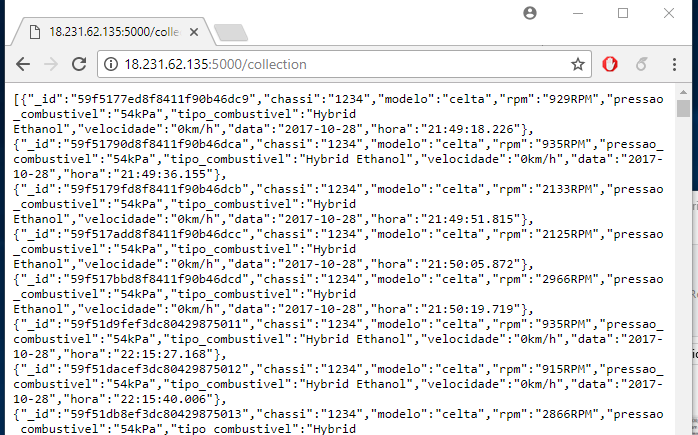
\includegraphics[scale=.68]{imagens/JSON_retornoWebservice.png}}\\
\makebox[\width]{Fonte: produzido pelo autor} \label{Fig:json_retorno_web}
\end{figure}

Por fim, foi testado com sucesso o consumo dos dados por meio de uma página web (Figura \ref{Fig:pagina_web_tabela_dados}), através de requisições utilizando o \textit{AJAX} do \textit{JQuery} pelo \textit{frontend}.

\begin{figure}[!ht]
\centering
\caption{Foto da página web estruturando em uma tabela os dados \textit{JSON}.} 
{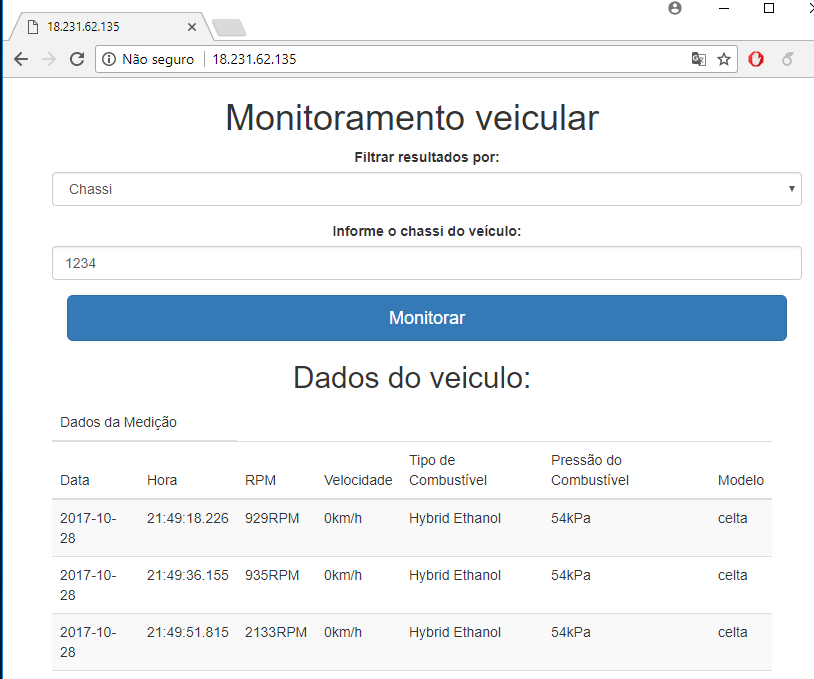
\includegraphics[scale=.68]{imagens/paginaweb_tabelaDados.png}}\\
\makebox[\width]{Fonte: produzido pelo autor} \label{Fig:pagina_web_tabela_dados}
\end{figure}